% !TeX spellcheck = en_US
\documentclass[10pt,a4paper,titlepage]{article}
\usepackage[latin1]{inputenc}
\usepackage{amsmath}
\usepackage{amsfonts}
\usepackage{amssymb}
\usepackage{makeidx}
\usepackage{graphicx}
\usepackage[left=2.00cm, right=2.00cm, top=2.00cm, bottom=2.00cm]{geometry}
\usepackage{tikz}
\usepackage{tikz-uml}
\linespread{1}
\usetikzlibrary{patterns}%for tikz https://tex.stackexchange.com/questions/54464/hatch-a-rectangle-in-tikz
%sources
\usepackage[backend=bibtex]{biblatex}
\bibliography{Thesis}
%Makes index browsable in pdf viewers and shows index in sidebar
\usepackage[bookmarks]{hyperref}
%Captions for figures in minipage
\usepackage{caption}

\author{Mikail Gedik}
\title{Thesis Paper}
%Ensures that \ref works with paragraphfs as intended
\setcounter{secnumdepth}{6}
\begin{document}
	\pagenumbering{roman}
	\maketitle
	\tableofcontents
	\listoffigures
	\clearpage
	\pagenumbering{arabic}
	
	\section{Abstract}
	This paper tackles the calculation of a few selected fractals and shines light on the core aspects I have implemented and furthermore optimized to use all the resources provided by the computer. My journey begins at a single threaded Java program and ends in a multi threaded C application able to make use graphics cards. Additionally, I will make an easy-to use yet powerful UI, which will enable even tech-unfamiliar people to use my software.
	\section{What are Fractals}
	Fractals are complex geometric shapes with special properties. But in contrast to normal finite Euclidean shapes (such as the circle, sphere, cube etc.), fractals are infinite. The angles and the lines of a cube are indifferent from the magnification. Fractals have the property that no matter how much they are magnified or zoomed into, the edges are never smooth but rough. New levels of detail will appear. Surprisingly, some fractals can even contain themselves. This property (well seen in the Sierpinski triangle, figure \ref{fig:sierpinski_triangle}) is called self-similarity. Although the self-similarity in this example is perfect, many fractals contain non-perfect copies of themselves. This can often be observed in nature, for example tree branches or snowflakes (figure \ref{fig:snowflake}).\\
	There are different types of fractals: geometric, algebraic and naturally occurring. Geometric and algebraic fractals are created by repeating a process over and over again. The Sierpinski triangle repeatedly cuts out the center piece of each black triangle \ref{fig:sierpinski_triangle_build}. The algebraic ones iterate have to iterate over an equation to determine its shape.\\
	While they were first conceptualized by Felix Hausdorff in 1918, the term fractal (from Latin fragmented, broken) was only coined in 1975 by mathematician Benoit B. Mandelbrot. A factor in this long time span were the invention of computers, which made the exploration of fractals much easier due to their impressive computation power. Mandelbrot used fractals as a tool to examine the stock market, but were also found to be useful in various fields like physical chemistry, fluid mechanics and physiology. \cite{FractalFoundation}, \cite{FractalFoundation}, \cite{britannica}.
	\begin{figure}[h]
		\caption{Sierpi?ski triangle \cite{Sierpinski}}
		\label{fig:sierpinski_triangle}
		\centering
		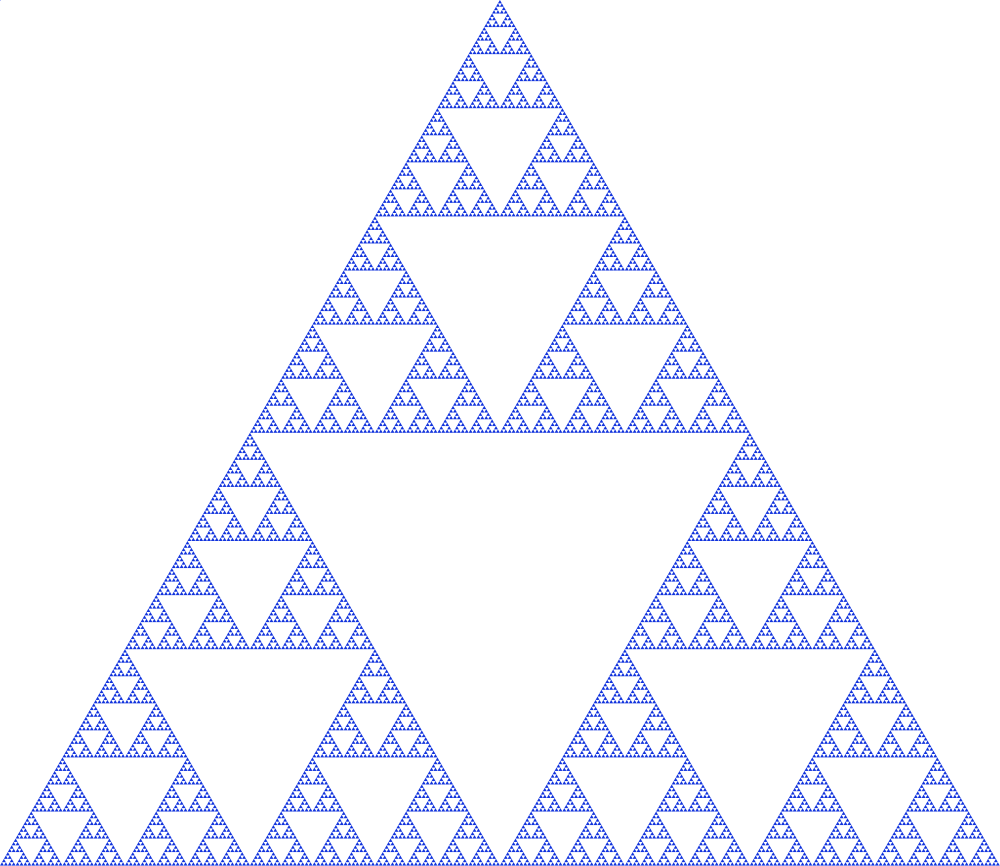
\includegraphics[width=0.5\textwidth]{"res/images/1000px-Sierpinski_triangle.svg.png"}
	\end{figure}
	\begin{figure}[h]
		\caption{Each branch of the snowflake creates new smaller branches \cite{wikipedia_snowflake}}
		\label{fig:snowflake}
		\centering
		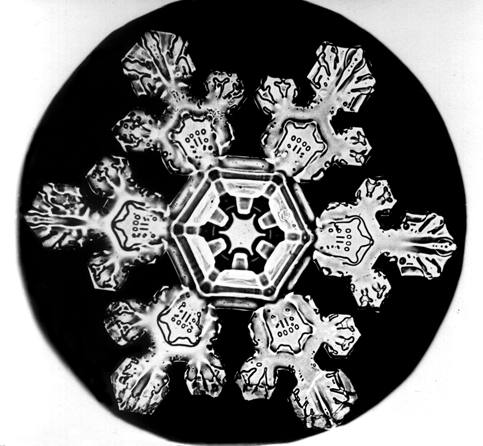
\includegraphics[width=0.5\textwidth]{"res/images/bentley_snowflake.jpg"}
	\end{figure}
	\begin{figure}[h]
		\caption{Creation of the Sierpinski triangle}
		\label{fig:sierpinski_triangle_build}
		\centering
		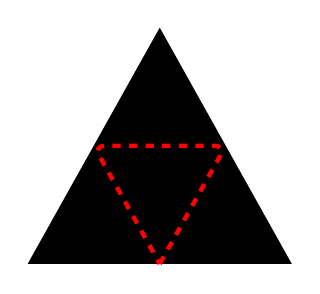
\begin{tikzpicture}[scale=3]
		\fill[black] (0,0) -- (1.118,0) -- (1.118/2, 1);
		
		\draw[rounded corners, dashed, red, ultra thick] (1.118/2, 0) -- (1.118/4*3,.5) -- (1.118/4, .5) -- (1.118/2, 0);
		\end{tikzpicture}
		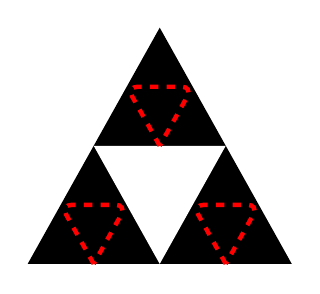
\begin{tikzpicture}[scale=3]
		\fill[black] (0,0) -- (1.118033989,0) -- (1.118033989/2, 1);
		\fill[white] (1.118/2, 0) -- (1.118/4*3,.5) -- (1.118/4, .5);
		
		\draw[rounded corners, dashed, red, ultra thick] (1.118/4*3, 0) -- (1.118/8*5,.25) -- (1.118/8*7, .25) -- (1.118/4*3, 0);
		\draw[rounded corners, dashed, red, ultra thick] (1.118/4, 0) -- (1.118/8,.25) -- (1.118/8*3, .25) -- (1.118/4, 0);
		\draw[rounded corners, dashed, red, ultra thick] (1.118/2, .5) -- (1.118/8*3,.75) -- (1.118/8*5, .75) -- (1.118/2, .5);
		\end{tikzpicture}
		
\begin{tikzpicture}[scale=3]
		\fill[black] (0,0) -- (1.118033989,0) -- (1.118033989/2, 1);
		
		\fill[white] (1.118/2, 0) -- (1.118/4*3,.5) -- (1.118/4, .5);
		
		\fill[white] (1.118/4*3, 0) -- (1.118/8*5,.25) -- (1.118/8*7, .25);
		\fill[white] (1.118/4, 0) -- (1.118/8,.25) -- (1.118/8*3, .25);
		\fill[white] (1.118/2, .5) -- (1.118/8*3,.75) -- (1.118/8*5, .75);
		\end{tikzpicture}
	\end{figure}
	
	%finite fractal contains infinity/self-similarity. occurs in nature. equally rough at all scales. not possible to understand with classical geometry\cite{FractalsForDummies}.\\
	%Never ending repeating branching pattern. (Infinitely complex). Made by repeating simple process often. Geometric fractals created by repeating simple process (sierpinski triangle). Algebraic fractals: repeat equation over and over \cite{FractalFoundation}:\\
	%complex geometric shapes. Concept by Felix Hausdorff 1918. Are distinct from classical/Euclidean geometry (square, circle, sphere etc.). spatially nonuniform phenomena in nature (coastlines, mountain ranges). Word fractal (Latin for "fragmented", "broken") by mathematician Benoit B. Mandelbrot. Fractals as tools for different fields (stock market). Self-similar objects have remain invariant under changes of scale: they have scaling symmetry. Fractal dimension vs. euclidean dimension, a noninteger. Fractals are used to simulate nature (e. g. tree branches)\cite{britannica}
	
	%mathematics used to use classical analysis
	%classical analysis cannot explain sets or functions which are too irregular
	%have therefore been ignored and labled as curiosity
	%New developement shows that irregular sets are better approximations of natural phenomens
	%Tipical properties of fractals:
	%self similarity, detailed microstructure, definition simple -> fractal complex, generated using recursion, no description possible using classic geometry, local geomtry not describable, size of set is infinity but size is zero
	%\cite{FalconerKennethJ1993FG:m}
	
	\section{The Mandelbrot Set}
	Although the most part of my thesis paper is dedicated to computer science the necessity arises to explain the most used fractal in my work. The Mandelbrot set was named after Benoit Mandelbrot, and is the first one to be called a fractal. In terms of properties, it is related to the Julia set, which is not a part of my work, albeit my program has the ability to display them. The Mandelbrot set is an algebraic fractal in the complex plane \(z = a + b i\). To find out which points are part of the set, we have to repeatedly apply the function \(z_{n+1} = z_{n}^2 + c\) to every point \(z\) in the plane. If the point diverges (or is known to diverge) as \(n\) approaches infinity, it is said to be outside the set. The most interesting points lie at the boundary of the set, as the edge is the most interesting part of any fractal.
	
	%named after benoit mandelbrot. related to julia set. choose complex number \(c\) and \(z_0\) and repeatedly put into equation \(z_n = z_{n+1} + c\). If \(z_n\) diverges, point not in fractal. Interesting points near boundary \cite{freeuk}
	\section{The Program}
	This section represents the core of my paper. The capabilities, structure and implementation are discussed in depth
	\subsection{Program Functionalities}
	\subsection{Structure}
	My program is separated in two halves, the GUI and core. While the latter is autonomous, the former is dependent on the core, as it must know its interface, which is the connecting bridge between them. The GUI can request or order a command through a command string or an integer, i. e. a character sequence or a number. The core answer these with a command result, which may also be an image.\\
	Because the core is detached from the GUI, I may also develop multiple GUIs for different needs. The GUI in the diagram below shows a possible version of window-oriented GUI, which is relatively modern and user-friendly, but for example useless in a command line environment. Thus I see the need to develop different GUIs.
	
	\begin{figure}
		\centering
		\label{fig:program_structure}
		\caption{Program structure}
		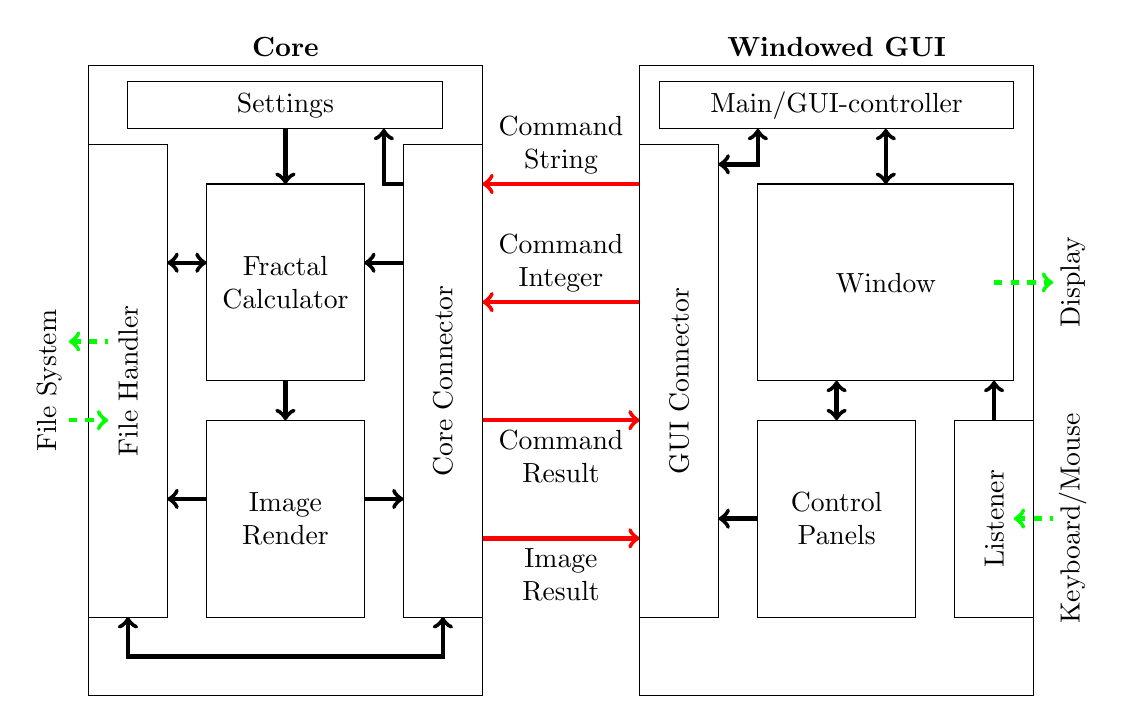
\begin{tikzpicture}
		%Front/Backend-connection
		\draw[red, ultra thick, <-] (5,6.5) -- (7,6.5);
		\node[above, align=center] at (6,6.5) {Command\\String};
		
		\draw[red, ultra thick, <-] (5,5) -- (7,5);
		\node[above, align=center] at (6,5) {Command\\Integer};
		
		\draw[red, ultra thick, ->] (5,3.5) -- (7,3.5);
		\node[below, align=center] at (6,3.5) {Command\\Result};
		
		\draw[red, ultra thick, ->] (5,2) -- (7,2);
		\node[below, align=center] at (6,2) {Image\\Result};
		
		%Backend
		\draw (0,0) rectangle (5,8);
		\node[above] at (2.5, 8) {\textbf{Core}};
		
		%Interface
		\draw (4,1) rectangle (5, 7);
		\node[rotate = 90] at(4.5, 4) {Core Connector};
		
		%Settings
		\draw (.5,7.2) rectangle (4.5, 7.8);
		\node at (2.5, 7.5) {Settings};
		
		%Fractal calculator
		\draw (1.5,4) rectangle (3.5, 6.5);
		\node[align=center] at (2.5, 5.25) {Fractal\\Calculator};
		
		%Image render
		\draw (1.5,1) rectangle (3.5, 3.5);
		\node[align=center] at (2.5, 2.25) {Image\\Render};
		
		%File handling
		\draw (0,1) rectangle (1, 7);
		\node[rotate = 90] at(.5, 4) {File Handler};
		
		%Arrows
		%Settings-Frac
		\draw[ultra thick, ->] (2.5, 7.2) -- (2.5, 6.5);
		%Int-Frac
		\draw[ultra thick, <-] (3.5, 5.5) -- (4, 5.5);
		%Frac-Image
		\draw[ultra thick, ->]  (2.5, 4) -- (2.5, 3.5);
		%Img-Int
		\draw[ultra thick, ->]  (3.5, 2.5) -- (4, 2.5);
		%Frac-File
		\draw[ultra thick, <->] (1.5, 5.5) -- (1, 5.5);
		%Image-File
		\draw[ultra thick, ->] (1.5, 2.5) -- (1, 2.5);
		%Settings-Int
		\draw[ultra thick, ->] (4, 6.5) -- (3.75, 6.5) -- (3.75, 7.2); 
		%Int-File
		\draw[ultra thick, <->] (4.5, 1) -- (4.5,.5) -- (.5,.5) -- (.5, 1);
		
		%File system
		\draw[green, ultra thick, dashed, ->] (-.25, 3.5) -- (.25, 3.5);
		\draw[green, ultra thick, dashed, <-] (-.25, 4.5) -- (.25, 4.5);
		\node[rotate = 90] at (-.5, 4) {File System};
		
		%Frontend
		\draw (7,0) rectangle (12,8);
		\node[above] at (9.5, 8) {\textbf{Windowed GUI}};
		
		%Interface
		\draw (7,1) rectangle (8, 7);
		\node[rotate = 90] at(7.5, 4) {GUI Connector};
		
		%Main
		\draw (7.25,7.2) rectangle (11.75, 7.8);
		\node at (9.5, 7.5) {Main/GUI-controller};
		
		%Window
		\draw (8.5,4) rectangle (11.75, 6.5);
		\node[align=center] at (10.125, 5.25) {Window};
		
		%Control Panels
		\draw (8.5,1) rectangle (10.5, 3.5);
		\node[align=center] at (9.5, 2.25) {Control\\Panels};
		
		%Listener
		\draw (11,1) rectangle (12, 3.5);
		\node[rotate = 90] at(11.5, 2.25) {Listener};
		
		%Arrows
		%Main-Win
		\draw[ultra thick, <->] (10.125 ,7.2) -- (10.125, 6.5);
		%List-Win
		\draw[ultra thick, ->] (11.5, 3.5) -- (11.5,4);
		%Ctr-Win
		\draw[ultra thick, <->] (9.5, 3.5) -- (9.5, 4);
		%Main-Interface
		\draw[ultra thick, <->] (8, 6.75) -- (8.5, 6.75) -- (8.5, 7.2);
		
		%Ctr-Interface
		\draw[ultra thick, <-] (8, 2.25) -- (8.5, 2.25);
		
		%Keyboard/Mouse
		\draw[green, ultra thick, dashed, ->] (11.5, 5.25) -- (12.25,5.25);
		\node[rotate = 90] at (12.5, 5.25) {Display};
		
		\draw[green, ultra thick, dashed, <-] (11.75, 2.25) -- (12.25, 2.25);
		\node[rotate = 90] at (12.5, 2.25) {Keyboard/Mouse};
		\end{tikzpicture}
	\end{figure}

	\subsubsection{Core}
	The core consists of multiple components or modules, which are tightly bound together. Each of them is responsible for a certain task and should not do anything else. The modules are only capable of communicating to each other and are isolated from the `outside', with the exception of the connector and file handler. The latter two interchange data with the UI or underlying file system.
	\paragraph{Settings}
	%Settingsmanager is simple list with keys (e.g name of the setting) and values. Some settings are relevant for rendering, some for the calculation. Some are variable, others are standart information like version
	The settings for calculation are either used directly for computation or as parameters for the program itself. Variables used during the computation could be for example the \(C\) in the Julia set, numerals such as the maximal number of iterations allowed during computation or the color function used when coloring the calculated set. Other more technical information regarding the system, for instance available RAM, CPU name or the version of the program, may also be stored there. Although the word settings suggest that these values are changeable too during runtime, they are not meant to change. To see the difference between mutable and immutable values, changeable ones are prefixed with \verb|setting|, while the others are prefixed with \verb|value|.
	\paragraph{Fractal Calculator}
	%Handles calculation and organizes multithreading 
	Upon receiving the command from the interface, the fractal calculator starts to calculate a set of points according to the parameters fetched from the settings module. After having created all necessary information to start the rendering process, the calculation's result is given either to the image render module or to the file handler. The fractal calculator is the core part of my thesis paper and I will spend most of my time tinkering with and finding optimizations for it.
	\paragraph{Image Render Module}
	%Creates images from the data
	
	The image render module creates images from the data calculated. A major advantage of this module is the buffering of data; Since the user will zoom in only gradually, new images created are often based on already used data. To make use of this, previously generated images are buffered and reused if possible.
	\subparagraph{Color Function}
	The color function maps the values of calculated points to colors. The simplest coloring is the in-out one, showing if a point has diverged or not. A more complex coloring method involves the amount of iterations a point had to take for its divergence, resulting in a much more colorful plot, and also showing the Mandelbrot's branches clearly.
	\paragraph{File Handler}
	The file handler abstracts the saving and reading process of fractals, videos or images. This module is the smallest one, since most of its implementation is already provided by the default library of Java.
	%Abstracts saving and reading from the file system
	\paragraph{Data Model}
	The data model is the one of the most complex parts of my project. One of the toughest nuts to crack was the intelligent allocation and distribution of data, which was necessary to have low access time when searching specific points or areas in the dataset. To achieve this, the data is logically split in multiple layers: the levels and clusters. A level is container for multiple clusters, which in turn contain the data. All levels cover the same area, but with a different density of clusters, resulting in a different precision. One more caveat was RAM usage; My first algorithm was simpler and less sophisticated, and started using a massive amount of RAM to precache not yet calculated points. Although this made fetching data faster, it was unusable since the application was bound to crash after zooming in only a little bit.\\
	\paragraph{Connector}
	%Connector handles calls for the core. Sorts, creates, destroys and handles whole backend. Makes sure that rendered area is calculated
	The connector manages calls from the UI to the backend, instructing the fractal calculator or image render module on what to do. Although this part is omittable since all the components could be called directly by the UI, I have added it because it abstracts and facilitates the usage of the core. Through this abstraction I have been able to make changes to the core without altering the UI.
	\subsubsection{GUI}
	The GUI (graphics user interface) is the mediator between the core and the user. It makes the program's capabilities, which are invoked through methods and functions, available to humans, only capable (without considering voice commands or touch screens) to interfere with the computer by mouse and keyboard. The GUI takes commands, which are issued by mouse clicks or keyboard strokes, and forwards them to the core. These commands usually yield a result, which is reported back to the GUI and shown to the user. For all this, a window is needed.
	\subsection{Implementation}
	This section sums up the central algorithms and structures which build my program.
	\subsubsection{Helper Classes}
	These structures do not contain any important algorithms or functionalities, but are used as wrappers for simple data. Since they are used often, I must make them trivial before being able to explain the more complex aspects of my program.
	\paragraph{Region}
	A the \verb|Region| class is a wrapper for a clip of the calculated set. It is defined by a start and end point. The coordinates are real floating point numbers, internally stored as primitive \verb|double|s. To avoid unintentional changes, the fields of the class are marked as final. Thus, there are only getter methods for the fields. To simplify the usage further, there are also methods to calculate the width and height of the clip.
	\paragraph{Logic Region}
	The \verb|LogicRegion| class has the same functionalities as the \verb|Region| class, but uses a different approach to store the data. Explaining the alternative method will be in vain without having read the section \ref{sec:data_management} regarding the data management, but may still be explained by using an example.
	Imagine a box filled with apples. The box and apples both have fixed dimensions, as shown in figure \ref{fig:apples_in_box} (page \pageref{fig:apples_in_box}). The box and apples are an analogy to my program, which uses levels and clusters. An area of this box can now be defined using two different methods. The more intuitive way would to make the measurements in centimeters, i. e. the green arrows; the region starts at the point \((8\text{cm},8\text{cm})\) and ends at the point \((24\text{cm}, 32\text{cm})\). No matter how big or small the apples are, the region stays the same. Another way to define the area, illustrated by blue arrows, employs another metric. Instead of centimeters apples are used, thus defining the start at \((2\text{apples},2\text{apples})\) and the end at \((5\text{apples},4\text{apples})\). Note that the apple at \((5\text{apples},4\text{apples})\) is not in the clip, although it is used to define the clip. This is because when referring to an apple, the reference point is always the lower left corner. Although it might seem unfit to define it this way, there is another reason to do this. To get the dimensions, one can now simply subtract the start from the end point, which would otherwise give a wrong result (\((5\text{apples},4\text{apples}) - (2\text{apples},2\text{apples}) = (3\text{apples},2\text{apples})\)).\\
	The logic region facilitates the access to clusters stored in a level by being able to directly access their position instead of having to deal with their absolute position. The implementation of this class is the same as the \verb|Region|, but it uses the \verb|int| instead of the \verb|double| type.
	\begin{figure}
		\centering
		\begin{minipage}{.5\textwidth}
			\captionof{figure}{Apples(red) in a box (black), as seen from above}
			\label{fig:apples_in_box}
			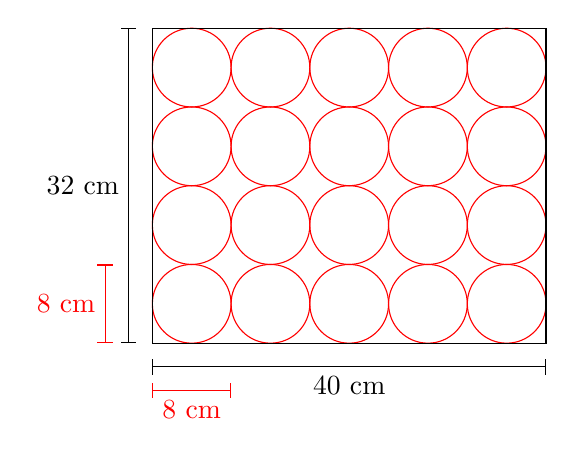
\begin{tikzpicture}
			\draw[|-|] (0,-.3) -- (2.5,-.3) node[below] {40 cm} -- (5,-.3);
			\draw[|-|] (-.3,0) -- (-.3, 2) node[left] {32 cm} -- (-.3,4);
			
			\draw[red, |-|] (0,-.6) -- (0.5,-.6) node[below] {8 cm} -- (1,-.6);
			\draw[red, |-|] (-.6,0) -- (-.6, .5) node[left] {8 cm} -- (-.6,1);
			
			\foreach \x in {0,1,2,3,4} {
				\foreach \y in {0,1,2,3} {
					\draw[red] (.5 + \x, .5 + \y) circle[radius=.5];
				}
			}
			\draw (0,0) rectangle (5,4);
			\end{tikzpicture}
		\end{minipage}
		\begin{minipage}{.4\textwidth}
			\captionof{figure}{Mesurements for normal region (green) vs. logic region(blue)}
			\label{fig:apples_in_box_with_region}
			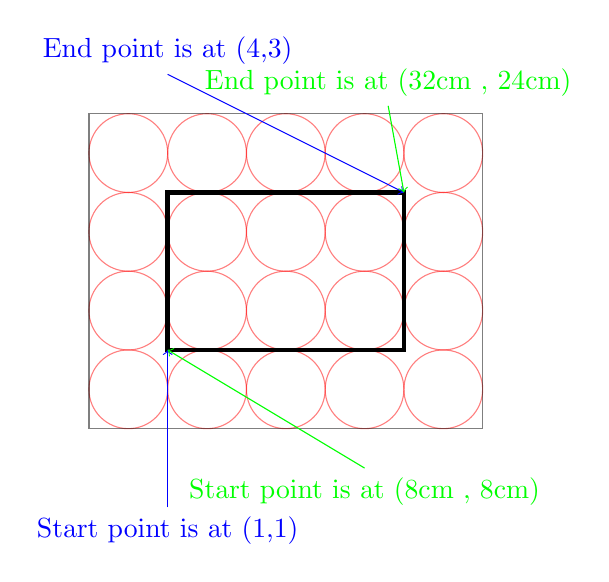
\begin{tikzpicture}
			\foreach \x in {0,1,2,3,4} {
				\foreach \y in {0,1,2,3} {
					\draw[opacity = .5, red] (.5 + \x, .5 + \y) circle[radius=.5];
				}
			}
			\draw[opacity = .5] (0,0) rectangle (5,4);
			
			\draw[ultra thick] (1,1) rectangle (4,3);
			
			\draw[->, blue] (1,-1) node[below] {Start point is at (1,1)} -- (1,1);
			\draw[->, green] (3.5,-.5) node[below] {Start point is at (8cm , 8cm)} -- (1,1);
			
			\draw[->, blue] (1,4.5) node[above] {End point is at (4,3)} -- (4,3);
			\draw[->, green] (3.8,4.1) node[above] {End point is at (32cm , 24cm)} -- (4,3);
			\end{tikzpicture}
		\end{minipage}
	\end{figure}

	\paragraph{Screen}
	The \verb|Screen| class represents a rasterized image with fixed dimensions. Internally, a \verb|int[]| array stores all the data. The class provides various methods used in basic image manipulation. I had initially written this class long ago for other projects, but since I needed a class with these functionalities I have recycled it and added it to this project.
	\subsubsection{Data Management}\label{sec:data_management}
	Data calculated can be stored in many ways, from simple arrays to complex databanks. To understand the approach I have taken on storing data, I will have to explain the way computers store memory.
	\paragraph{Accessing RAM}
	It has become trivial knowledge that computers work with zeroes and ones, but to understand the problems faced in storing data, I have to explain the principles a little further. To remember the values that my program has calculated, it stores them in the RAM. The RAM (random access memory) is essentially a gigantic collection of cells, each able to hold a single byte (one byte corresponds to eight bits, or eight zeroes or ones). To gain access to the memory, every cell has its own address, which is (on modern operating systems/computers) a 64 bit number. Since a 64 bit number is quite long, they are usually represented in hexadecimal format. In figure \ref{fig:memory_cells1} (page \pageref{fig:memory_cells1}) there is a schematic drawing of five memory cells, each labeled with their address (to make the numbers shorter, the addresses' length is only 16 bit). Each of these cells can hold a value $V$ between zero and 255 (that being the highest number a byte can represent). How these cells are exactly accessed, set up and managed is quite interesting and complicated, but I will not discuss this in detail since it is not relevant for my work.\\
	\subparagraph{Storing numbers}
	Storing an number is quite simple. Figure \ref{fig:memory_cells2} (page \pageref{fig:memory_cells2}) shows two numbers, one eight and one sixteen bit, stored in the RAM. The eight bit number can have values from 0 to 255, since it cannot represent more values. As bigger numbers are required, the system reserves multiple cells and treats their value as a single one. Storing the number 2234, \((00001000\text{ }10111010)_2\) in binary format, requires two cells. The number is split between the cells, one holding the value \((00001000)_2 (= (8)_{10})\) and the other \((10111010)_2(=(186)_{10})\). Nowadays computers usually use 32 or 64 bit numbers, requiring four or eight bytes per number.
	
	\subparagraph{Storing lists}
	The next step to storing single numbers is storing a list of numbers. Lists, often called arrays, are nothing more than many numbers lined up behind each other. Figure \ref{fig:memory_cells3} (page \pageref{fig:memory_cells3}) shows a list with five 1 byte elements. In computer science, list usually start at the index zero instead of one because it usually is easier to access them, as I will shortly explain. The zeroth element has the address \(2E\), the first \(2F\) and so on. Because each element's address can be easily expressed by the previous', it is only necessary to remember the zeroth's. Assuming \(A_{0}\) is the zeroth's address, the \(n\)th elements' can be determined using the formula \(A_{n}=A_{0} + n \times s\), where \(s\) is the amount of bytes each element needs, in this case one. Giving an example, the third elements address \(A_{3}\) is equals to \(2E + 3 \times 1 = 31\).
	\cite{howstuffworks}
	\begin{figure}
		\centering
		\caption{Memory cells, with addresses in hexadecimal format}
		\label{fig:memory_cells1}
		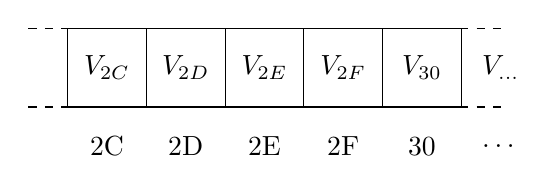
\begin{tikzpicture}
			\draw[dashed] (-.5, 1) -- (5.5, 1);
			\draw[dashed] (-.5, 0) -- (5.5, 0);
			\draw[step = 1] (0,0) grid (5,1);
			
			\node at (0.5, .5) {$V_{2C}$};
			\node at (1.5, .5) {$V_{2D}$};
			\node at (2.5, .5) {$V_{2E}$};
			\node at (3.5, .5) {$V_{2F}$};
			\node at (4.5, .5) {$V_{30}$};
			\node at (5.5, .5) {$V_{\dots}$};
			
			\node at (.5, -.5) {2C};
			\node at (1.5, -.5) {2D};
			\node at (2.5, -.5) {2E};
			\node at (3.5, -.5) {2F};
			\node at (4.5, -.5) {30};
			\node at (5.5, -.5) {\dots};
		\end{tikzpicture}
	\end{figure}
	
	\begin{figure}
		\centering
		\caption{Memory cells storing a numbers}
		\label{fig:memory_cells2}
		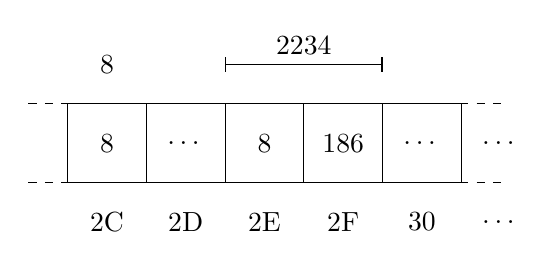
\begin{tikzpicture}
		\draw[dashed] (-.5, 1) -- (5.5, 1);
		\draw[dashed] (-.5, 0) -- (5.5, 0);
		\draw[step = 1] (0,0) grid (5,1);
		
		\node at (.5, 1.5) {8};
		
		\draw[|-|] (2, 1.5) -- (3, 1.5) node[above] {2234} -- (4, 1.5);
		
		\node at (.5, .5) {8};
		\node at (1.5, .5) {$\dots$};
		\node at (2.5, .5) {8};
		\node at (3.5, .5) {186};
		\node at (4.5, .5) {$\dots$};
		\node at (5.5, .5) {\dots};
		
		
		\node at (.5, -.5) {2C};
		\node at (1.5, -.5) {2D};
		\node at (2.5, -.5) {2E};
		\node at (3.5, -.5) {2F};
		\node at (4.5, -.5) {30};
		\node at (5.5, -.5) {\dots};
		\end{tikzpicture}
	\end{figure}
	
	\begin{figure}
		\centering
		\caption{Memory cells storing an array}
		\label{fig:memory_cells3}
		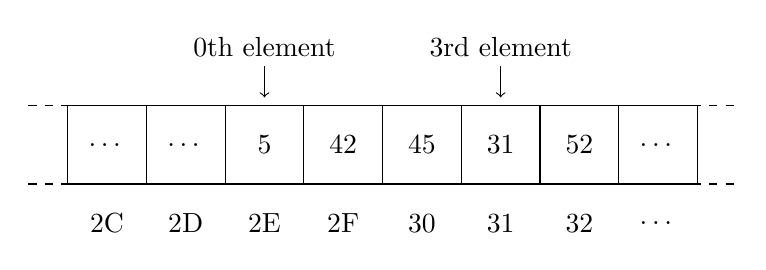
\begin{tikzpicture}
		\draw[dashed] (-.5, 1) -- (8.5, 1);
		\draw[dashed] (-.5, 0) -- (8.5, 0);
		\draw[step = 1] (0,0) grid (8,1);
		
		\draw[->] (2.5, 1.5) node[above] {0th element} -- (2.5, 1.1);
		
		\draw[->] (5.5, 1.5) node[above] {3rd element} -- (5.5, 1.1);
		
		\node at (.5, .5) {\dots};
		\node at (1.5, .5) {\dots};
		\node at (2.5, .5) {5};
		\node at (3.5, .5) {42};
		\node at (4.5, .5) {45};
		\node at (5.5, .5) {31};
		\node at (6.5, .5) {52};
		\node at (7.5, .5) {\dots};
						
		\node at (.5, -.5) {2C};
		\node at (1.5, -.5) {2D};
		\node at (2.5, -.5) {2E};
		\node at (3.5, -.5) {2F};
		\node at (4.5, -.5) {30};
		\node at (5.5, -.5) {31};
		\node at (6.5, -.5) {32};
		\node at (7.5, -.5) {\dots};
		\end{tikzpicture}
	\end{figure}

	\subparagraph{Storing an Image in RAM}
	Since the RAM is a one dimensional space, allocating one dimensional objects like numbers, lists or similar things is quite easy. It suffices to know the size of the elements to access one. Storing multidimensional objects requires two map them to a single dimension.\\
	In case of an image, each pixel has two indexes denoting the locations on the abscissa and ordinate axes. The pixels are thus describe by two identifiers, making them two dimensional. To store them in RAM, the two indexes have to be converted into a single identifier. Figure \ref{fig:2d_to_1d} (page \pageref{fig:2d_to_1d}) shows this transition. On the left, each pixel \(P_{x,y}\) is described using two indices \(x, y\), while on the right the pixels \(P_{i}\) are described by the single index \(i\). The goal is to find a way to transform the indices \(x, y\) to a single index. By defining \(i = x + 3 \times y\), both indices are mapped to a single one.
	
	\begin{figure}
		\centering
		\caption{Mapping a two dimensional image to a single dimension}
		\label{fig:2d_to_1d}
		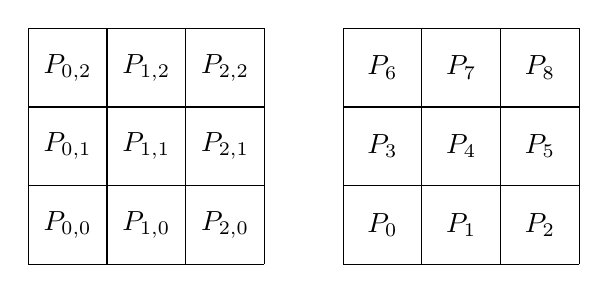
\begin{tikzpicture}
			\draw (0,0) grid (3,3);
			\foreach \y in {0,1,2} {
				\foreach \x in {0,1,2} {
					\node at (\x + .5, \y + .5) {$P_{\x,\y}$};
				}
			}
		
			\draw (4,0) grid (7,3);
			\foreach \x in {0,1,2} {
				\node at (4 + \x + .5, .5) {$P_{\x}$};
			}
			\foreach \x in {3,4,5} {
				\node at (1 + \x + .5, 1 + .5) {$P_{\x}$};
			}
			\foreach \x in {6,7,8} {
				\node at (-2 + \x + .5, 2 + .5) {$P_{\x}$};
			}
		\end{tikzpicture}
	\end{figure}
	
	\subsubsection{The Dataset}
	The dataset is responsible for the storage, access and management of values calculated by my program. Implementation wise, the central parts are located in the \verb|DataSet| class, which contains all methods relevant for the management. The classes \verb|Level|, \verb|Cluster| and \verb|Value| help sorting the data in logically aligned subsets. Figure \ref{fig:dataset_hierarchy} (page \pageref{fig:dataset_hierarchy}) shows the components hierarchically. The dataset contains levels and these contain cluster which are made of values.
	
	\begin{figure}
		\centering
		\caption{The structure of the dataset}
		\label{fig:dataset_hierarchy}
		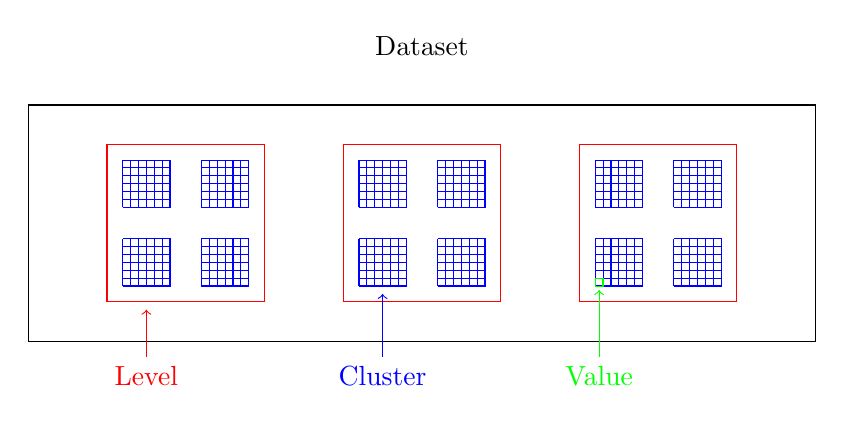
\begin{tikzpicture}
			
			\draw (0, 0) rectangle (10,3);
			\foreach \level in {0,3,6} {
				\draw[red] (\level+1, .5) rectangle (\level+3, 2.5);
				\foreach \cx/\cy in {0/0,0/1,1/0,1/1} {
					\draw[blue, step=.1] (\level+1 + \cx + .2, \cy+.7) grid (\level+.8 + \cx + 1.01 , \cy + 1.3);
				}
			}
			\draw[green] (7.2, .7) rectangle (7.3,.8);
			\node[above] at (5, 3.5) {Dataset};
			\draw[red,   ->] (1.5, -.2) node[below] {Level} -- (1.5, .4);
			\draw[blue,  ->] (4.5, -.2) node[below] {Cluster} -- (4.5, .6);
			\draw[green, ->] (7.25, -.2) node[below] {Value} -- (7.25, .65);
		\end{tikzpicture}
	\end{figure}
	\paragraph{Basic understanding}
	All values calculated are stored in the \verb|Value| class. This class is a wrapper for a single value. The job of the dataset is to store these in a way that they are quickly accessible. The first viable solution is to store them in a single big list. This however has the drawback that the entire list has to be searched for a value. The solution to this was to group values in an area together to form a so-called cluster. These are then again sorted by their precision into different levels. Figure \ref{fig:dataset_actual} (page \pageref{fig:dataset_actual}) shows how the data is stored, taking the actual position of the data into account. 
	
	\begin{figure}
		\centering
		\caption{The actual of the dataset shown with the Cartesian coordinate system, taking position into account\newline The dataset/level is black, clusters are blue and values are green}
		\label{fig:dataset_actual}
		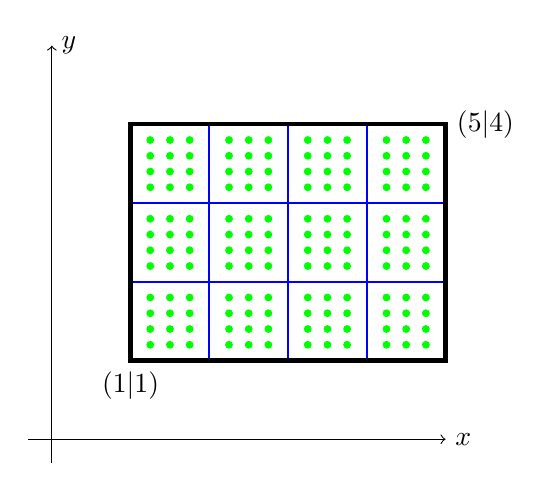
\begin{tikzpicture}
			\draw[->] (-1,-1.3) -- (-1,4) node[right] {$y$};
			\draw[->] (-1.3,-1) -- (4,-1) node[right] {$x$};
			\foreach \cx  in {0,1,2,3} {
				\foreach \cy  in {0,1,2} {
					\draw[thick, blue] (\cx,\cy) rectangle (\cx+1,\cy+1);
					\foreach \px  in {0,1,2} {
						\foreach \py  in {0,1,2,3} {
							\fill[green] ({\cx + \px * 0.25 + .25}, {\cy + \py * 0.2 + .2}) circle[radius=.05];
						}
					}
				}
			}
			\draw[ultra thick] (0,0) node[below] {$(1|1)$} rectangle (4,3) node[right] {$(5|4)$};
		\end{tikzpicture}
	\end{figure}
	
	\subparagraph{Value}
	The value wraps a single value. It contains no other data, not even the location which the data corresponds to. These are determined by the position of the cluster and the index of the value in the cluster.
	\subparagraph{Cluster}
	A cluster is a collection of values. As seen in figure \ref{fig:dataset_actual} (page \pageref{fig:dataset_actual}), a the values contained are in a rectangle. The width can be measured in two ways: either the absolute width \(w_{\text{cls,abs}}\), referring to the width of cluster's area, or the logical width \(w_{\text{cls,log}}\), expressing the width in amount of values. In the figure, \(w_{\text{cls,log}} = 3\) and \(w_{\text{cls,abs}} = 1\) can easily be interpreted. The same rule can be applied to the height, expressed by \(h_{\text{cls,log}}\) and \(h_{\text{cls,abs}}\).\\
	In a dataset all clusters are required to have the same logical dimensions. The absolute width and height, as well as the position, can vary.
	\subparagraph{Level}
	The level is a list of clusters. Similar the aforementioned, it has two different ways to measure its dimension. An absolute, referring to area of the set it covers (\(w_{\text{lev,abs}}\) and \(h_{\text{lev,abs}}\)), and a logical, involving the amount of clusters it contains. The main difference is that all levels in a dataset have the same absolute dimensions. In figure \ref{fig:dataset_different_levels} (page \pageref{fig:dataset_different_levels}), three levels of a dataset are shown. All span from the point \((1|1)\) to \((4|3)\). However, the amount of clusters they fit is different. The table shows the values that change with the depth \(d\), which describes how many values a level contains.
	\begin{figure}
		\centering
		\caption{Different levels in the same dataset}
		\label{fig:dataset_different_levels}
		\begin{minipage}{.4\textwidth}
			\centering
			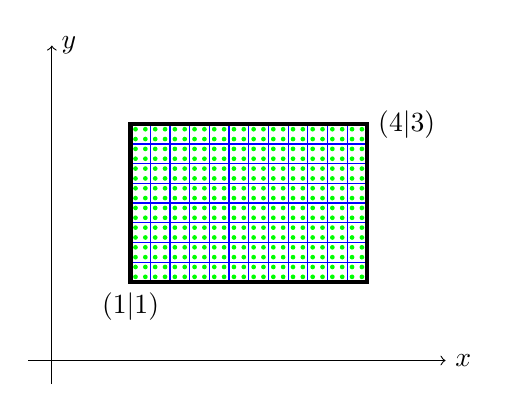
\begin{tikzpicture}
				\draw[->] (-1,-1.3) -- (-1,3) node[right] {$y$};
				\draw[->] (-1.3,-1) -- (4,-1) node[right] {$x$};
				\draw[step=.25,blue] (0,0) grid (3,2);
				\foreach \x in {0,...,23} {
					\foreach \y in {0,...,15} {
						\fill[green] (.125*.5 + 0.125 * \x, .125*.5 + 0.125 * \y) circle[radius=.03];
					}
				}
				\draw[ultra thick] (0,0) node[below] {$(1|1)$} rectangle (3,2) node[right] {$(4|3)$};
			\end{tikzpicture}
		\end{minipage}%
		\begin{minipage}{.4\textwidth}
			\centering
			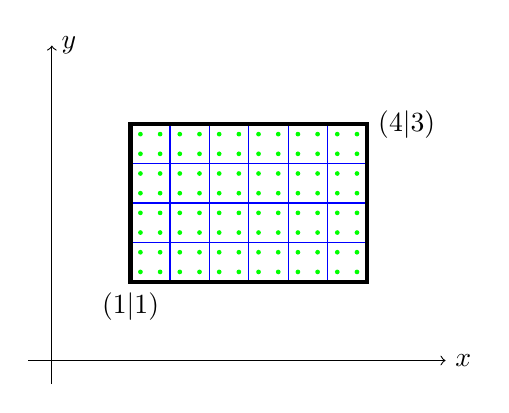
\begin{tikzpicture}
				\draw[->] (-1,-1.3) -- (-1,3) node[right] {$y$};
				\draw[->] (-1.3,-1) -- (4,-1) node[right] {$x$};
				\draw[step=.5,blue] (0,0) grid (3,2);
				\foreach \x in {0,...,11} {
					\foreach \y in {0,...,7} {
						\fill[green] (.125 + 0.25 * \x, .125 + 0.25 * \y) circle[radius=.03];
					}
				}
				\draw[ultra thick] (0,0) node[below] {$(1|1)$} rectangle (3,2) node[right] {$(4|3)$};
			\end{tikzpicture}
		\end{minipage}
		\begin{minipage}{.4\textwidth}
			\centering
			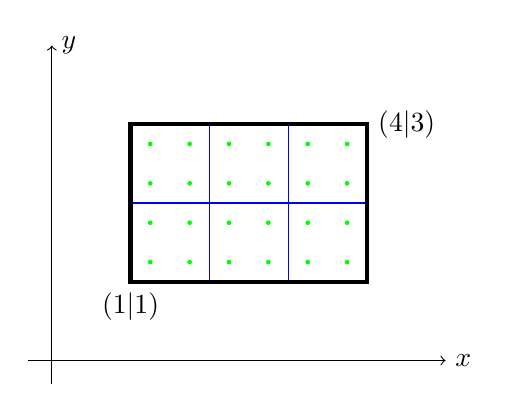
\begin{tikzpicture}
				\draw[->] (-1,-1.3) -- (-1,3) node[right] {$y$};
				\draw[->] (-1.3,-1) -- (4,-1) node[right] {$x$};
				\draw[step=1,blue] (0,0) grid (3,2);
				\foreach \x in {0,...,5} {
					\foreach \y in {0,...,3} {
						\fill[green] (.25 + 0.5 * \x, .25 + 0.5 * \y) circle[radius=.03];
					}
				}
				\draw[ultra thick] (0,0) node[below] {$(1|1)$} rectangle (3,2) node[right] {$(4|3)$};
			\end{tikzpicture}
		\end{minipage}
		\begin{minipage}{.4\textwidth}
			\centering
				\begin{tabular}{c|c|c|c|c}
					&\(w_{\text{lev,abs}}\)&\(h_{\text{lev,abs}}\)&\(w_{\text{lev,log}}\)&\(h_{\text{lev,log}}\)\\\hline
					Level 1&3&2&3&2\\\hline
					Level 2&3&2&6&4\\\hline
					Level 3&3&2&12&8\\
				\end{tabular}		
		\end{minipage}
	\end{figure}
	
	\subparagraph{Dataset}
	The dataset stores all levels, clusters and values and provides methods to access them. It defines all the parameters used, such as \(h_{\text{lev,abs}}\) or \(w_{\text{cls,log}}\).
	\paragraph{Implementation}
	
	\subsubsection{Image Generation}
	%take advantage of data arrangement, since sorted in clusters and levels and thus by precision
	%naive algorithm: search for nearest datapoint
	A less vital but still important aspect of my work is the visualization of the data. It is crucial to consider the way the data is stored when performing access-intense tasks, such as this. A more naive approach of mine search the whole dataset for each pixel colored, resulting in abysmal performance. By using a more sophisticated algorithm, the data can be directly mapped to the image without searching long for it. This section will go sequentially through all the steps taken.
	\paragraph{Image Parameters}
	\begin{figure}
		\centering
		\caption{Function Signature to create images}
		\label{fig:image_signature}
		\begin{verbatim}
		public Screen createScreen(int minPixelWidth, int minPixelHeight, Region region,
		                int threads, long maxWaitingTime)
		\end{verbatim}
	\end{figure}
	To know what type of image the program has to create, parameters have to be passed to the function called. As seen in figure \ref{fig:image_signature} (page \pageref{fig:image_signature}), the first two refer to the (minimal) image constraints in pixels, \verb|region| describes the region of the fractal to render. \verb|threads| indicates the maximal, although not minimal, amount of CPU threads used to create the image, and \verb|maxWaitingTime| indicates how long the image creation can take before it is aborted to avoid blocking the application in case of an error, infinty loop or deadlock (although neither is likely to happen at all).\\
	The returned \verb|Screen| has at least the dimensions given by the parameters, but is very likely to surpass them. Due to the mapping of the pixels the actually displayed region might vary by at most a single pixel, but I have deemed that negligible.	
	\paragraph{Preparing the rendered Area}
	In figure \ref{fig:region_over_dataset}, the starting point of the problem is visible. A clip of the dataset has to be mapped onto the red region. Using the given dimensions of the red area, the necessary precision of the datapoints can be derived. Through the precision, we can calculate the necessary level and get the smallest logic region which can fit the red area inside it (figure \ref{fig:logic_region_over_dataset}, page \pageref{fig:logic_region_over_dataset}). The logic region is needed to know from which level and place (index to be exact) in the dataset the data has to be queried, rending a long search for the datapoints redundant. The precision of the level is always better or equal to the precision of the requested image.	
	\begin{figure}
	\centering
	\caption{The dataset region(black) and the requested region (red)}
	\label{fig:region_over_dataset}
		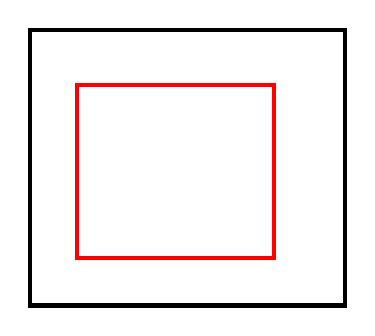
\begin{tikzpicture}
			\draw[ultra thick,black, step=.5] (0,0) rectangle (4,3.5);
			\draw[ultra thick,red] (0.6, .6) rectangle (3.1, 2.8);
		\end{tikzpicture}
	\end{figure}
	
	\begin{figure}
		\centering
		\caption{The level, its clusters and the logic region in green}
		\label{fig:logic_region_over_dataset}
		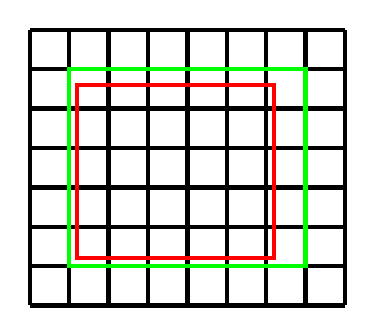
\begin{tikzpicture}
			\draw[ultra thick,black, step=.5] (0,0) grid (4, 3.5);
			\draw[ultra thick,red] (0.6, .6) rectangle (3.1, 2.8);
			\draw[ultra thick, green] (.5, .5) rectangle(3.5,3);
		\end{tikzpicture}
	\end{figure}
	\paragraph{Image allocation}
	Instead of allocating an empty image with the specified dimensions and filling it directly with data, the allocated image has the dimensions of the logical area. I have illustrated this in figure \ref{fig:logic_region_and_requested_area} (page \ref{fig:logic_region_and_requested_area}). The logic cluster width and height are both 5, the logical area has the width and height of 3. The requested area lies unaligned with the rest in the middle, with a width of 5 and a height of 6. As seen in the image, the region where data is fetched from has a greater precision as the red requested area; The values in the dataset lie closer to each other than in the area.\\
	Following this example, the allocated image width is the logical cluster width times the logical region width (\(4 \times 5 = 20\)), and the image height is the logical cluster height times the logical area height (\(4 \times 6 = 24\)). The dimensions are measured in pixels. After it has been created, it can be immediately filled with data , which is a rather easy process since the pixels are by definition perfectly aligned with the data. In my program, this interim result is called \verb|ImageResult| and is cached for later usage(see section \ref{par:paragraph_image_creation_buffering}, page \pageref{par:paragraph_image_creation_buffering}) \\
	After the image has been populated by the values, it can be cropped to the requested area. But as seen in figure \ref{fig:cropping the area} (page, \pageref{fig:cropping the area}), the cropped image's properties are not as requested. The image is wider and taller than asked for, but this is a rather minor problem since it does not degrade the quality and can be easily corrected by scaling the image down. A bigger problem regarding the accuracy is that the returned clipping is slightly bigger than requested.
	
	\begin{figure}
		\centering
		\caption{The logical area (green) with clusters and values (blue), and the requested region (red) with pixels}
		\label{fig:logic_region_and_requested_area}
		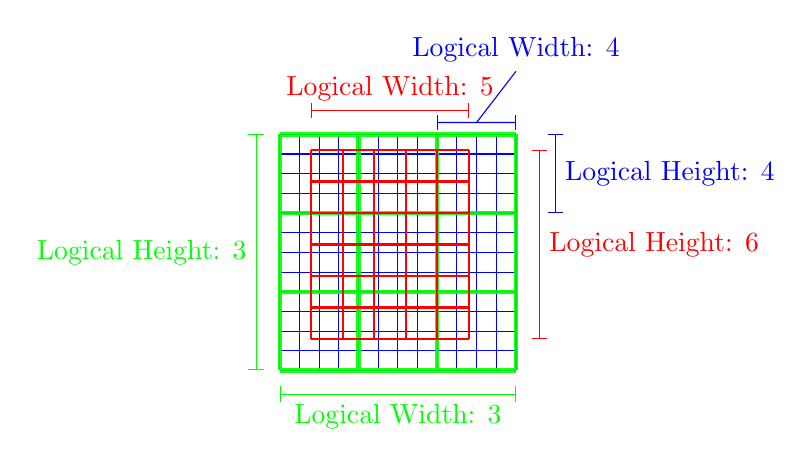
\begin{tikzpicture}
			\draw[|-|,green] (0, -.3) -- (1.5, -.3) node[below] {Logical Width: 3}-- (3, -.3);
			\draw[|-|,green] (-.3, 0) -- (-.3, 1.5) node[left] {Logical Height: 3}-- (-.3, 3);
			
			\draw[|-|,red] (0.4, 3.3) -- (1.4, 3.3) node[above] {Logical Width: 5}-- (2.4, 3.3);
			\draw[|-|,red] (3.3, 0.4)-- (3.3, 1.6) node[right] {Logical Height: 6}-- (3.3, 2.8);
			
			\draw[|-|,blue] (2, 3.15) -- (2.5, 3.15) -- (3, 3.8) node[above] {Logical Width: 4} -- (2.5,3.15)-- (3, 3.15);
			\draw[|-|,blue] (3.5, 2)-- (3.5, 2.5) node[right] {Logical Height: 4}-- (3.5, 3);
			
			\foreach \x in {0,1,2} {
				\foreach \y in {0,1,2} {
					\draw[blue, step=.25] (\x, \y) grid (\x +1, \y + 1);
				}
			};
			\draw[ultra thick, green, step=1, opacity=.9] (0, 0) grid (3,3);
			\draw[thick, red, step=.4] (0.4, 0.4) grid (0.4 + .4 * 5, 0.4 + .4 * 6);
		\end{tikzpicture}
	\end{figure}
	
	\begin{figure}
		\centering
		\caption{Cropping the image to the area given by the parameters}
		\label{fig:cropping the area}
		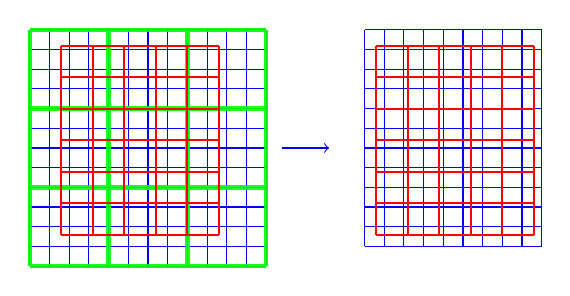
\begin{tikzpicture}			
		\foreach \x in {0,1,2} {
			\foreach \y in {0,1,2} {
				\draw[blue, step=.25] (\x, \y) grid (\x +1, \y + 1);
			}
		};
		\draw[ultra thick, green, step=1, opacity=.9] (0, 0) grid (3,3);
		\draw[thick, red, step=.4] (0.4, 0.4) grid (0.4 + .4 * 5, 0.4 + .4 * 6);
		
		\draw[->, blue] (3.2, 1.5) -- (3.8, 1.5);
		\draw[blue, step=.25] (4.24999, .25) grid (4 + 2.5, 3);
		\draw[thick, red, step=.4] (4.3999, 0.4) grid (4.4 + .4 * 5, 0.4 + .4 * 6);
		
		\end{tikzpicture}
	\end{figure}
	
	\paragraph{Buffering} \label{par:paragraph_image_creation_buffering}
	As mentioned above, generated \verb|ImageResult|s are cached for further usage. The reason becomes quite clear when thinking of the usual navigation in fractals. The user will often slowly zoom into a section of the set. This means for the render engine that it will create many images with a nearly identical area, thus being in the same logical area. Hence having a buffer filled with previously generated \verb|ImageResult|s can reduce the rendering time by much. Searching the buffer for a match takes place after knowing the logical area an image needs to be rendered. It is then checked against every entry in it, and if a suitable \verb|ImageResult| is found, it is taken and used instead of creating a new one from scratch. If this is not the case, a new \verb|ImageResult| has to strenuously be created and is afterwards added to the buffer.\\
	An issue encountered with buffering is the increasing RAM usage. Since the buffer contains only data which can be recreated at medium cost, it is not necessary to let it grow infinitely. Limiting its size leads to less RAM usage, but potentially a higher performance impact.\\ The buffer is only useful in cases where the roughly the same area is rendered often, such as zooming in or moving our a little. As soon as the area is moved around or zoomed in too much, thus requiring a new logical area or new depth respectively, a new \verb|ImageResult| has to be created.
	\subsubsection{GUI}
	\section{Workflow and Major Version History}
	
	\section{Reflection}
	Programming an application of this size has come with many unexpected challenges which are tied to the nature of computer science. These challenges have, when not accounted for, caused either several delays in my time schedule or forced me to not implement a feature. One of the most banal and trivial hardships encountered are logical errors in the code, causing either simple misbehavior or runtime crashes. These can be prevented 
	
	
	
	
	
	
	
	
	
	
	\clearpage
	\appendix
	\printbibliography
\end{document}